% !Mode:: "TeX:UTF-8"
% !TEX program  = xelatex

%\documentclass{cumcmthesis}
\documentclass[withoutpreface,bwprint]{cumcmthesis} %去掉封面与编号页

\usepackage{url}   % 网页链接
\usepackage{subcaption} % 子标题
\title{全国大学生数学建模竞赛编写的 \LaTeX{} 模板}
\tihao{A}
\baominghao{4321}
\schoolname{XX大学}
\membera{}
\memberb{向左}
\memberc{哈哈}
\supervisor{老师}
\yearinput{2017}
\monthinput{08}
\dayinput{22}

\title{一维非齐次热传导方程的向后Euler格式}
\begin{document}
	\maketitle
	~\\
	~\\
	
	作业:
	$$
	\left\{
	\begin{array}{lcl}
	\dfrac{\partial{u}}{\partial{t}}=\dfrac{\partial^{2}{u}}{\partial{x}^{2}} &,&0 \leq x \leq 1,0 \leq t \leq 1 \\
	
	u(x,0)=e^x &, & 0 \leq x \leq 1 \\
	
	u(0,t)=e^t,u(1,t)=e^{1+t},&, &0 \leq t \leq 1
	\end{array}
	\right.
	$$
	
	

	
	
	该问题的精确解为$ u(x,t)=e^{x+t}$.
	
	定义误差为$$ E_{\infty}(h,\tau)=\max \limits_{1 \leq i \leq m-1 \atop 1 \leq k \leq n } |u(x_{i},t_{k})-u_{k}^k)| $$
	
	用向后Euler格式求下述问题的数值解并对数值解、精度和误差阶进行相应的数值分析。

	
	~\\
	~\\
	
	解:
	
	将xm等分,将tn等分, 记$h=\dfrac{1}{m},\tau=\dfrac{1}{n}$

	$x_i=ih,0 \leq i \leq m$
	
	$t_k=k \tau,0 \leq k \leq n$
	
	向后Euler差分格式为
	$$
	\left\{
	\begin{array}{lcl}
	-\gamma u_{i-1}^k+(1+2 \gamma) u_i^k- \gamma u_{i+1}^k=u_i^{k-1}+\tau f(x_i,t_k) \\
	u_i^0=e^{x_{i}} \\
	u_0^k=e^{t_k},u_m^k=e^{1+t_k} \\
	\end{array}
	\right.
	$$
	
	其中,$1 \leq i \leq m-1,1 \leq k \leq n,\gamma=\dfrac{\tau}{h^2}$
	
	$f(x_i,t_k)=0$
	

    
	写成矩阵形式$Au=f$
	
	其中
	$$
	A=
	\begin{bmatrix}
	1+2\gamma & -\gamma \\
	-\gamma & 1+2\gamma & -\dfrac{\gamma}{2} \\
	& \ddots & \ddots & \ddots \\
	 & & 	-\gamma & 1+2\gamma
	\end{bmatrix}
	$$
	
	
	$$u^k=[u_1^k,u_2^k,\cdots,u_{m-1}^k]^T$$.
	
	$$f=[u_1^{k-1}+\gamma u_0^k,u_2^{k-1},\cdots,u_{m-2}^{k-1},u_{m-1}^{k-1}+\gamma u_m^k]^T$$.
	
	
	解方程,由第k层的值,能够求出第k+1层的值。
	
	~\\
	~\\
	
	
	\textbf{解题程序运行于Matlab 2018a.}
	
	当$\tau=\dfrac{1}{100},h=\dfrac{1}{10}$时,t=1处的数值解和精确解见图\ref{fig:f1},从图像上看很接近。
	\begin{figure}
		\centering
		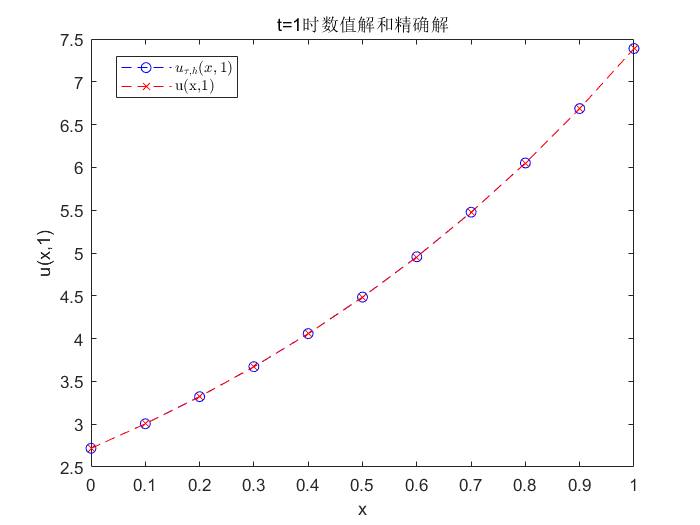
\includegraphics[width=0.7\linewidth]{figures/f1}
		\caption{t=1处的数值解和精确解}
		\label{fig:f1}
	\end{figure}

	当$\tau=\dfrac{1}{100},h=\dfrac{1}{10}$时,取x=0.5,不同t处的值见表\ref{tab:1},
	当层数越深时,误差越大,这是因为,每一次由k层求解k+1层时都有误差,随着t的增大,误差不断累积,越来越大,
	到t=1处误差变得最大。
	\begin{table}[htbp]
		\centering
		\caption{x=0.5时,不同t处的数值解、精确解和误差}
		\begin{tabular}{ccccc}
			\toprule[1.5pt]
			k     & t     & 数值解   & 精确解   & 误差 \\
			\midrule[1pt]
			10    & 0.1   & 1.822891  & 1.822119  & 7.7174E-04 \\
			20    & 0.2   & 2.014927  & 2.013753  & 1.1743E-03 \\
			30    & 0.3   & 2.226965  & 2.225541  & 1.4242E-03 \\
			40    & 0.4   & 2.461227  & 2.459603  & 1.6237E-03 \\
			50    & 0.5   & 2.720096  & 2.718282  & 1.8140E-03 \\
			60    & 0.6   & 3.006178  & 3.004166  & 2.0124E-03 \\
			70    & 0.7   & 3.322344  & 3.320117  & 2.2271E-03 \\
			80    & 0.8   & 3.671759  & 3.669297  & 2.4625E-03 \\
			90    & 0.9   & 4.057922  & 4.055200  & 2.7219E-03 \\
			100   & 1     & 4.484697  & 4.481689  & 3.0084E-03 \\
			\bottomrule[1.5pt]
		\end{tabular}%
		\label{tab:1}%
	\end{table}%

	
	
	取不同$\tau$ 和 $h$时,t=1处的误差见图\ref{fig:f2},步长越小,误差也越小。
	\begin{figure}
		\centering
		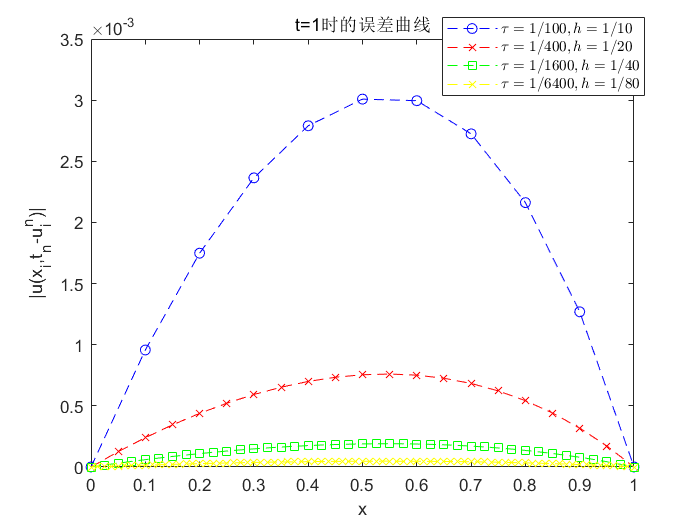
\includegraphics[width=0.7\linewidth]{figures/f2}
		\caption{不同步长下的误差}
		\label{fig:f2}
	\end{figure}
	
	

	取不同步长时,误差和误差比见图用向后Euler格式, $\tau$变为原来的4倍,$h$变为原来的2倍,误差会变为原来的4倍,
	符合$O(\tau+h^2)$的截断误差
	
	% Table generated by Excel2LaTeX from sheet 'Sheet1'
	\begin{table}[htbp]
		\centering
		\caption{取不同步长时的误差和误差比}
		\begin{tabular}{ccc}
			\toprule[1.5pt]
			$h,\tau$   & $E_{\infty}(h,\tau)$ & $E_{\infty}(2h,4\tau)/E_{\infty}(h,\tau)$ \\
			\midrule[1pt]
			1/100,1/10 & 3.0084E-03 & * \\
			1/400,1/20 & 7.6035E-04 & 3.956615  \\
			1/1600,1/40 & 1.9023E-04 & 3.997046  \\
			1/6400,1/80 & 4.7566E-05 & 3.999261  \\
			\bottomrule[1.5pt]
		\end{tabular}%
		\label{tab:2}%
	\end{table}%
\end{document}